\documentclass[11pt,a4paper]{article}
\usepackage[margin=18mm]{geometry}
\usepackage{amsmath,amssymb,mathtools}
\usepackage{booktabs,array,enumitem}
\usepackage[dvipsnames]{xcolor}
\usepackage{listings}
\usepackage{tikz}
\usetikzlibrary{arrows.meta,positioning,decorations.pathmorphing}
\usepackage[most]{tcolorbox}
\usepackage{hyperref}
\hypersetup{colorlinks=true,urlcolor=MidnightBlue,linkcolor=MidnightBlue}
\setlength{\parindent}{0pt}
\setlength{\parskip}{4pt}
\newcommand{\course}{Computational Methods in Physics}
\newtcolorbox{keybox}{colback=RoyalBlue!5,colframe=RoyalBlue!65!black,boxrule=.7pt,arc=2mm}
\newtcolorbox{checkbox}{colback=ForestGreen!5,colframe=ForestGreen!55!black,boxrule=.7pt,arc=2mm}
\newtcolorbox{aibox}{colback=BurntOrange!7,colframe=BurntOrange!80!black,boxrule=.7pt,arc=2mm}
\lstdefinestyle{matlabstyle}{
  language=Matlab,
  basicstyle=\ttfamily\footnotesize,
  keywordstyle=\color{RoyalBlue!75!black},
  commentstyle=\color{ForestGreen!55!black},
  stringstyle=\color{BurntOrange!80!black},
  numbers=left,
  numberstyle=\scriptsize\color{black!50},
  numbersep=5pt,
  frame=single,
  rulecolor=\color{RoyalBlue!25},
  backgroundcolor=\color{RoyalBlue!3},
  showstringspaces=false,
  columns=fullflexible,
  keepspaces=true,
  breaklines=true
}
\begin{document}

{\large\textsc{\course}}\\[-2pt]
{\small Learning Note \textbar\ Week 4}\par\vspace{4pt}
{\LARGE\bfseries Eigenproblems and Physical Modes}\par\vspace{3pt}
\textit{An eigenproblem becomes physically meaningful when its eigenvalues, eigenvectors, units, and validation checks are connected back to measurable collective motion.}

\begin{keybox}
\textbf{Physical question.} How can two coupled masses move in special collective patterns that preserve their relative shape while oscillating at characteristic frequencies?
\end{keybox}

\section*{Learning outcomes}
By the end of this week, you should be able to:
\begin{enumerate}[nosep,leftmargin=5mm]
  \item derive a two-degree-of-freedom oscillator model from Newton's second law;
  \item formulate the generalized eigenproblem $\mathbf{K}\boldsymbol{\phi}=\lambda\mathbf{M}\boldsymbol{\phi}$;
  \item connect $\lambda$ to angular frequency and frequency with correct units;
  \item normalize and interpret eigenvectors as physical mode shapes without over-interpreting arbitrary scale or sign;
  \item validate computed modes using symmetry, analytic references, eigen-equation residuals, orthogonality, and limiting cases; and
  \item identify one preferred bounded capstone question and one alternate candidate with feasible validation evidence.
\end{enumerate}

\section*{1. From simultaneous motion to special patterns}
Coupled systems have several coordinates that influence one another. In a two-mass oscillator, a displacement of mass 1 changes the force on mass 2 through the coupling spring, and vice versa. Most initial conditions produce a mixture of motions, but some displacement patterns are special: the entire shape simply scales up and down while oscillating at one characteristic frequency. These are the \textbf{normal modes}.

\begin{center}
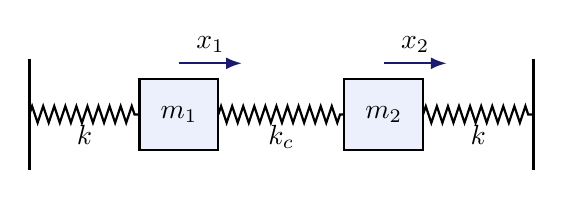
\begin{tikzpicture}[x=1cm,y=1cm,thick]
  \draw[very thick] (0,0)--(0,1.4);
  \draw[decorate,decoration={zigzag,segment length=4pt,amplitude=3pt}] (0,0.7)--(1.4,0.7);
  \draw[fill=RoyalBlue!10] (1.4,0.25) rectangle (2.4,1.15);
  \node at (1.9,0.7) {$m_1$};
  \draw[decorate,decoration={zigzag,segment length=4pt,amplitude=3pt}] (2.4,0.7)--(4.0,0.7);
  \draw[fill=RoyalBlue!10] (4.0,0.25) rectangle (5.0,1.15);
  \node at (4.5,0.7) {$m_2$};
  \draw[decorate,decoration={zigzag,segment length=4pt,amplitude=3pt}] (5.0,0.7)--(6.4,0.7);
  \draw[very thick] (6.4,0)--(6.4,1.4);
  \node[below] at (0.7,0.7) {$k$};
  \node[below] at (3.2,0.7) {$k_c$};
  \node[below] at (5.7,0.7) {$k$};
  \draw[-{Latex[length=2mm]},MidnightBlue] (1.9,1.35)--(2.7,1.35); \node[above] at (2.3,1.35) {$x_1$};
  \draw[-{Latex[length=2mm]},MidnightBlue] (4.5,1.35)--(5.3,1.35); \node[above] at (4.9,1.35) {$x_2$};
\end{tikzpicture}
\end{center}

\begin{checkbox}
\textbf{Predict before computing.} For two equal masses and identical outer springs, sketch one mode where the masses move together and one where they move oppositely. Which should have the larger frequency? Explain using deformation of the coupling spring.
\end{checkbox}

\section*{2. Derive the equations of motion}
Let both masses equal $m$, the two outer springs equal $k$, and the coupling spring equal $k_c$. Measure $x_1$ and $x_2$ from static equilibrium and take rightward displacement as positive. For small undamped motion,
\begin{align}
 m\ddot{x}_1 &= -(k+k_c)x_1+k_cx_2,\\
 m\ddot{x}_2 &= k_cx_1-(k+k_c)x_2.
\end{align}
Move the restoring terms to the left and collect the coordinates:
\begin{equation}
 \underbrace{\begin{bmatrix}m&0\\0&m\end{bmatrix}}_{\mathbf{M}\;(\mathrm{kg})}
 \underbrace{\begin{bmatrix}\ddot{x}_1\\\ddot{x}_2\end{bmatrix}}_{\ddot{\mathbf{x}}\;(\mathrm{m\,s^{-2}})}+
 \underbrace{\begin{bmatrix}k+k_c&-k_c\\-k_c&k+k_c\end{bmatrix}}_{\mathbf{K}\;(\mathrm{N\,m^{-1}})}
 \underbrace{\begin{bmatrix}x_1\\x_2\end{bmatrix}}_{\mathbf{x}\;(\mathrm{m})}=0.
\end{equation}
The off-diagonal terms encode the coupling. Their negative sign is not a MATLAB convention; it comes from the restoring force created by relative displacement.

\section*{3. Harmonic motion turns the model into an eigenproblem}
For one normal mode, assume
\begin{equation}
 \mathbf{x}(t)=\boldsymbol{\phi}\cos(\omega t),
\end{equation}
where $\boldsymbol{\phi}$ is a fixed displacement pattern. Then
\begin{equation}
 \ddot{\mathbf{x}}(t)=-\omega^2\boldsymbol{\phi}\cos(\omega t).
\end{equation}
Substitution into $\mathbf{M}\ddot{\mathbf{x}}+\mathbf{K}\mathbf{x}=0$ gives
\begin{equation}
 (\mathbf{K}-\omega^2\mathbf{M})\boldsymbol{\phi}=0,
\end{equation}
or equivalently
\begin{equation}
 \boxed{\mathbf{K}\boldsymbol{\phi}=\lambda\mathbf{M}\boldsymbol{\phi}},
 \qquad \lambda=\omega^2.
\end{equation}
This is a \textbf{generalized eigenproblem}. Since stiffness divided by mass has units $(\mathrm{N\,m^{-1}})/\mathrm{kg}=\mathrm{s^{-2}}$, the eigenvalue has units $\mathrm{s^{-2}}$. Therefore
\begin{equation}
 \omega=\sqrt{\lambda}\quad(\mathrm{rad\,s^{-1}}),
 \qquad f=\frac{\omega}{2\pi}\quad(\mathrm{Hz}).
\end{equation}

\begin{aibox}
\textbf{Common interpretation error.} The eigenvalue is not the frequency in hertz. For this mechanical formulation, the eigenvalue is $\omega^2$. Taking a square root and then dividing by $2\pi$ is part of the physical interpretation, not cosmetic unit conversion.
\end{aibox}

\section*{4. Baseline symmetric system}
Use
\begin{equation}
 m=0.50\,\mathrm{kg},\qquad k=20\,\mathrm{N\,m^{-1}},\qquad k_c=10\,\mathrm{N\,m^{-1}}.
\end{equation}
The generalized eigenproblem can be solved directly in MATLAB:
\begin{lstlisting}[style=matlabstyle,caption={Generalized eigenproblem for the two-mass oscillator}]
M_kg = diag([0.50 0.50]);
K_Npm = [30 -10; -10 30];

[modeRaw,D] = eig(K_Npm,M_kg);
[lambda_per_s2,idx] = sort(diag(D));
modeRaw = modeRaw(:,idx);

omega_radps = sqrt(lambda_per_s2);
frequency_Hz = omega_radps/(2*pi);
\end{lstlisting}
The reference values are
\begin{equation}
 \lambda_1=40\,\mathrm{s^{-2}},\qquad \lambda_2=80\,\mathrm{s^{-2}},
\end{equation}
\begin{equation}
 \omega_1=6.32456\,\mathrm{rad\,s^{-1}},\qquad
 \omega_2=8.94427\,\mathrm{rad\,s^{-1}},
\end{equation}
and
\begin{equation}
 f_1=1.00658\,\mathrm{Hz},\qquad f_2=1.42353\,\mathrm{Hz}.
\end{equation}

\section*{5. Eigenvectors are relative mode shapes}
For the symmetric system, the two physical patterns are proportional to
\begin{equation}
 \boldsymbol{\phi}_1\propto\begin{bmatrix}1\\1\end{bmatrix},
 \qquad
 \boldsymbol{\phi}_2\propto\begin{bmatrix}1\\-1\end{bmatrix}.
\end{equation}
Mode 1 is \textbf{in phase}: both masses move together, so the coupling spring does not change length. Its frequency therefore depends only on $k/m$. Mode 2 is \textbf{out of phase}: the coupling spring is repeatedly stretched and compressed, increasing the effective restoring action and therefore the frequency.

An eigenvector has arbitrary nonzero scale. MATLAB may return $[-1,-1]^T$ instead of $[1,1]^T$; these represent the same physical mode. Normalize before comparing shapes, for example by setting the largest absolute component to one. The sign may also be reversed for consistent display.

\section*{6. Symmetry provides an analytic validation case}
Substitute the expected symmetry patterns directly into the equations. For the in-phase mode, $x_1=x_2$ and the coupling spring is unstretched:
\begin{equation}
 \omega_1^2=\frac{k}{m}=40\,\mathrm{s^{-2}}.
\end{equation}
For the out-of-phase mode, $x_2=-x_1$:
\begin{equation}
 \omega_2^2=\frac{k+2k_c}{m}=80\,\mathrm{s^{-2}}.
\end{equation}
These results exactly match the numerical eigenvalues for the baseline parameters. This is stronger evidence than merely observing that MATLAB completed without an error.

\section*{7. Residual and orthogonality answer different questions}
For each computed eigenpair, form the residual
\begin{equation}
 \mathbf{r}_i=\mathbf{K}\boldsymbol{\phi}_i-\lambda_i\mathbf{M}\boldsymbol{\phi}_i.
\end{equation}
A useful scaled residual is
\begin{equation}
 \rho_i=\frac{\|\mathbf{r}_i\|_2}{\|\mathbf{K}\|_2\|\boldsymbol{\phi}_i\|_2+|\lambda_i|\|\mathbf{M}\|_2\|\boldsymbol{\phi}_i\|_2}.
\end{equation}
This tests whether the eigenpair satisfies the assembled matrices. It does \emph{not} prove that the matrices were derived correctly.

For a symmetric conservative system with distinct modes, mass-normalized eigenvectors satisfy
\begin{equation}
 \boldsymbol{\Phi}^T\mathbf{M}\boldsymbol{\Phi}\approx\mathbf{I}.
\end{equation}
This gives a structurally different check from the eigen-equation residual.

\begin{center}
\small
\begin{tabular}{>{\raggedright\arraybackslash}p{.24\linewidth}>{\raggedright\arraybackslash}p{.33\linewidth}>{\raggedright\arraybackslash}p{.33\linewidth}}
\toprule
\textbf{Evidence} & \textbf{Question answered} & \textbf{Important limitation}\\ \midrule
Symmetry / analytic result & Does the model reproduce a known special case? & Applies only when its assumptions hold\\
Eigen residual & Does the eigenpair satisfy the assembled matrices? & Can be tiny for the wrong matrices\\
Mass orthogonality & Are distinct conservative modes structurally consistent? & Depends on model symmetry and definiteness\\
Limiting case & Does the result approach known behaviour as a parameter changes? & Requires a trustworthy limit\\ \bottomrule
\end{tabular}
\end{center}

\section*{8. Coupling strength creates frequency splitting}
For the symmetric model,
\begin{equation}
 \omega_1^2=\frac{k}{m},\qquad
 \omega_2^2=\frac{k+2k_c}{m}.
\end{equation}
Increasing $k_c$ therefore leaves the in-phase frequency unchanged while increasing the out-of-phase frequency. The separation between the two natural frequencies is a measurable signature of coupling.

The limiting case $k_c\rightarrow0$ is especially useful. Then the masses become independent and the two eigenvalues are equal:
\begin{equation}
 \lambda_1=\lambda_2=\frac{k}{m}.
\end{equation}
This repeated eigenvalue is called a \textbf{degeneracy}. At degeneracy, individual eigenvectors are not unique: any independent basis spanning the same two-dimensional eigenspace is acceptable. Therefore, demanding one exact pair of vectors from MATLAB is not a valid test.

\section*{9. Breaking symmetry changes the mode shapes}
Now keep $m_1=0.50\,\mathrm{kg}$ but increase $m_2$ to $0.75\,\mathrm{kg}$ while retaining $k=20\,\mathrm{N\,m^{-1}}$ and $k_c=10\,\mathrm{N\,m^{-1}}$. The frequencies become approximately
\begin{equation}
 f_1=0.88401\,\mathrm{Hz},\qquad f_2=1.32346\,\mathrm{Hz}.
\end{equation}
The mode shapes are no longer exact $[1,1]^T$ and $[1,-1]^T$ patterns. Unequal inertia changes the relative amplitudes, so the simple symmetric analytic formula no longer applies. Use the generalized eigen-equation residual, mass orthogonality, positive squared frequencies, and physically reasonable parameter trends instead.

\begin{aibox}
\textbf{Responsible AI use.} AI may help translate derived equations into MATLAB, but it can confuse $\lambda$, $\omega$, and $f$, mishandle eigenvector sign or normalization, and overstate residual evidence. Record accepted, modified, or rejected suggestions and the independent checks used.
\end{aibox}

\section*{10. Practical transfer and capstone progression}
The practical starts from the symmetric baseline and makes two controlled changes:
\begin{enumerate}[nosep,leftmargin=6mm]
  \item vary $k_c$ to observe frequency splitting and the zero-coupling degeneracy; and
  \item increase one mass to break symmetry and interpret the new mode shapes.
\end{enumerate}
For each change, predict a trend, compute evidence, validate it, and explain the physics rather than collecting numbers without a purpose.

By the end of Week 4, nominate one preferred capstone question and one alternate. State the physical system, controllable input, observable output, likely method, required data or parameters, and at least two independent checks. The choice remains provisional until Week 06.

\section*{Three takeaways}
\begin{enumerate}[nosep,leftmargin=6mm]
  \item The generalized eigenproblem comes from the equations of motion; $\lambda=\omega^2$, not frequency in hertz.
  \item Eigenvectors describe relative mode shape, so overall scale and sign are arbitrary.
  \item Trust requires layered evidence from analytic cases, residuals, orthogonality, and limiting behaviour.
\end{enumerate}

\begin{keybox}
\textbf{Preparation for the practical.} Complete the Week 04 Individual Practical Check --- Quiz in Google Classroom. Bring your derived two-mass equations and be ready to solve, validate, vary coupling, break symmetry, and record two capstone candidates.
\end{keybox}

\end{document}
